\documentclass[tikz,dvipsnames]{standalone}
\usetikzlibrary{backgrounds}
\usetikzlibrary{calc,positioning}

\begin{document}
 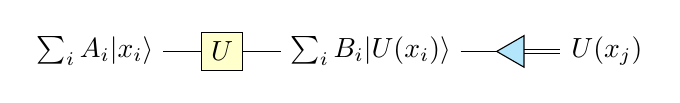
\begin{tikzpicture}[
    show background rectangle,
    tight background=0,
    background rectangle/.style={fill=white},
 ]
    \node (X) {$\sum_i A_i|x_i\rangle$};
    \node at (3.5,0) (Y) {$\sum_i B_i|U(x_i)\rangle$};
    \node at (6.5,0) (Z) {$U(x_j)$};
    \coordinate (P) at ($(Y)+(1.6,0)$);
    \coordinate (Q) at ($(P)+(0.2,0)$);
    \draw (X) -- node[fill=Yellow!20,draw]{$U$}  (Y) -- (P);
    \draw (Q) ++(0,+0.03) -- ++(0.6,0);
    \draw (Q) ++(0,-0.03) -- ++(0.6,0);
    \filldraw[fill=cyan!30] (P) -- ++(30:0.4) -- ++(270:0.4) -- cycle;
    
\end{tikzpicture}
\end{document}
